\documentclass[../../main.tex]{subfiles}
\begin{document}
\begin{oframed}
  \subfile{problem}
\end{oframed}

{\bf [解答]}

\paragraph{(1)}

\begin{figure}[htb]
  \centering
  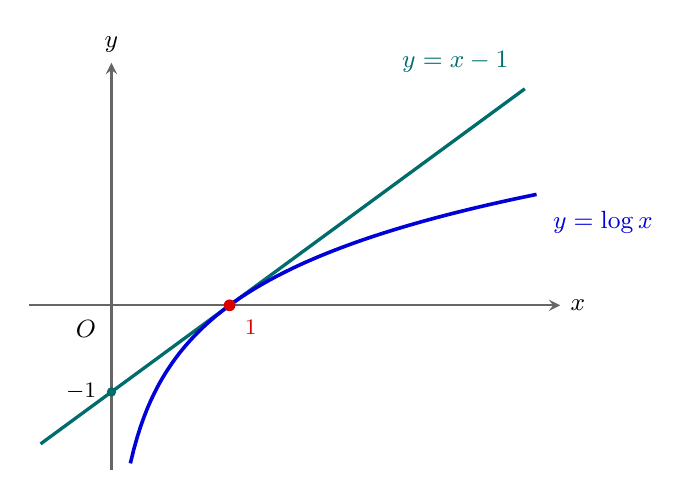
\begin{tikzpicture}[x=1.5cm, y=1.1cm, >=stealth, every node/.style={font=\small}]
    % 座標軸
    \draw[->, thick, gray!80!black] (-0.7, 0) -- (3.8, 0) node[right, black] {$x$};
    \draw[->, thick, gray!80!black] (0, -1.9) -- (0, 2.8) node[above, black] {$y$};
    \node[below left=2pt] at (0, 0) {$O$};

    % y = x - 1 と y = log x
    \draw[line width=1.2pt, teal!85!black, domain=-0.6:3.5]
    plot (\x, {\x - 1}) node[above left=2pt] {$y = x - 1$};
    \draw[line width=1.3pt, blue!85!black, domain=0.16:3.6, samples=120]
    plot (\x, {ln(\x)}) node[below right=2pt] {$y = \log x$};

    % y 切片 (0, -1) と接点 (1, 0)
    \node[circle, fill=teal!85!black, inner sep=1.2pt] at (0, -1) {};
    \node[left=2pt, font=\footnotesize] at (0, -1) {$-1$};
    \node[circle, fill=red!85!black, inner sep=1.5pt] at (1, 0) {};
    \node[below right=2pt, font=\footnotesize, red!85!black] at (1, 0) {$1$};
  \end{tikzpicture}
  \caption{$y=x-1$ と $y=\log x$ のグラフ}
\end{figure}

新しく
\begin{align}
  f(x) = x-1-\log x \quad (x>0) \label{eq:1}
\end{align}
とおくと，$f(x) \ge 0$を示せば良い．一階微分は
\begin{align}
  f'(x)=1-\dfrac{1}{x}
\end{align}
だから$f(x)$の増減表は以下のようになる．

\begin{table}[htb]
  \centering
  \caption{$f(x) = x - 1 - \log x$ の増減表（括弧は極限値）}
  \renewcommand{\arraystretch}{1.3}
  \begin{tabular}{c|ccccc}
    \hline
    $x$     & $(0)$      & $\cdots$   & $1$       & $\cdots$   & $(\infty)$ \\ \hline
    $f'(x)$ &            & $-$        & $0$       & $+$        &            \\ \hline
    $f(x)$  & $(\infty)$ & $\searrow$ & 極小 $0$  & $\nearrow$ & $(\infty)$ \\ \hline
  \end{tabular}
\end{table}

従って$f(x)$は$x=1$で最小値$f(1)=0$をとるから
\begin{align}
  f(x) \ge 0 \iff \log x\leqq x-1
\end{align}
が成り立つ．よって題意は示された．\qed

\paragraph{(2)}

与えられた積分を
\begin{align}
  I_n = n\int_{1}^{2}\log\left(\dfrac{1+x^{1/n}}{2}\right)dx \label{eq:2}
\end{align}
とおく．$t=x^{1/n}$とおくと$t^n=x$より$\dfrac{dx}{dt}=nt^{n-1}$で，$x:1\to2$の時$t:1\to 2^{1/n}$だから置換積分より
\begin{align}
  I_n
  & = n\int_{1}^{2^{1/n}}\log \left(\dfrac{1+t}{2}\right) \dfrac{dx}{dt} dt \\
  & = n\int_{1}^{2^{1/n}}\log \left(\dfrac{1+t}{2}\right) nt^{n-1} dt  \\
  & = n^2\int_{1}^{2^{1/n}}\log \left(\dfrac{1+t}{2}\right) t^{n-1} dt
\end{align}
となる．さらに部分積分を用いて
\begin{align}
  I_n
  & = n\left[\log \left(\dfrac{1+t}{2}\right) \cdot t^n \right]_{1}^{2^{1/n}}
  - n\int_{1}^{2^{1/n}} \dfrac{1}{1+t}t^n dt \\
  & = 2n \log \left(\dfrac{1+2^{1/n}}{2}\right)
  - n\int_{1}^{2^{1/n}} \dfrac{1}{1+t}t^n dt \label{eq:3}
\end{align}
を得る．この$n\to\infty$での極限を個別に考える．

まず第1項は$g(x)=\log\left(\dfrac{1+2^x}{2}\right)$，$x=\dfrac{1}{n}$とおくと$n\to\infty$の時$x\to 0$であって
\begin{align}
  (\text{第1項})
  &= 2n \log \left(\dfrac{1+2^{1/n}}{2}\right)
  = 2\dfrac{\log\left(\dfrac{1+2^x}{2}\right)}{x} \\
  &= 2\dfrac{g(x)-g(0)}{x}
  \xrightarrow{x\to 0} 2g'(0) \\
  &= \left. 2\dfrac{2^x \log 2 }{1+2^x}\right|_{x=0}
  = \log 2 \label{eq:4}
\end{align}
である．

次に第2項は区間$[1,2^{1/n}]$で
\begin{align}
  \dfrac{1}{1+2^{1/n}} \le \dfrac{1}{1+t} \le \dfrac{1}{2}
\end{align}
だから両辺に$nt^n$をかけて同区間で積分すると
\begin{align}
  n\int_{1}^{2^{1/n}}\dfrac{t^n}{1+2^{1/n}} dt \le (\text{第2項}) \le n\int_{1}^{2^{1/n}}\dfrac{t^n}{2} dt
\end{align}
を得る．両辺を積分して
\begin{align}
  & \dfrac{n}{1+2^{1/n}}\left[\dfrac{t^{n+1}}{n+1}\right]_{1}^{2^{1/n}}
  \le (\text{第2項})
  \le \dfrac{n}{2}\left[\dfrac{t^{n+1}}{n+1}\right]_{1}^{2^{1/n}} \\
  \therefore
  & \dfrac{n}{n+1}\dfrac{1}{1+2^{1/n}}\left[2^{(1+1/n)}-1\right]
  \le (\text{第2項})
  \le \dfrac{n}{2(n+1)}\left[2^{(1+1/n)}-1\right]
\end{align}
を得る．この両辺は$n\to\infty$の極限で$\dfrac{1}{2}$に収束するから挟み撃ちの定理から
\begin{align}
  \lim_{n\to\infty}(\text{第2項}) = \dfrac{1}{2}
\end{align}
である．

以上を\cref{eq:3}に代入して求める極限値は
\begin{align}
  \lim_{n\to\infty}I_n = \log 2 - \dfrac{1}{2}
\end{align}
である．

{\bf [解説]}

この問題は大学数学の範囲を使って積分と極限を交換すると一発で答えは出る．
答案には使えないが検算の手法として覚えておきたい．
\begin{align}
  \lim_{n\to\infty}n\int_1^2\log\dfrac{1+x^{1/n}}{2}\,dx
  &=\int_1^2\lim_{n\to\infty}n\log\dfrac{1+x^{1/n}}{2}\,dx \\
  &= \dfrac{1}{2}\int_1^2\log x\,dx\\
  &=\log2-\dfrac{1}{2}
\end{align}
となって解答と同じ値がでる．

% TODO: この手の問題の考え方の解説をしたい．うまく言語化できないんだけど，どうやって1/n次のオーダーを取り出すかをうまく説明したい
% TODO: 積分の部分を拡大した図が欲しいな．

\end{document}
